\documentclass[14pt]{extbook}
\usepackage{multicol, enumerate, enumitem, hyperref, color, soul, setspace, parskip, fancyhdr} %General Packages
\usepackage{amssymb, amsthm, amsmath, latexsym, units, mathtools} %Math Packages
\everymath{\displaystyle} %All math in Display Style
% Packages with additional options
\usepackage[headsep=0.5cm,headheight=12pt, left=1 in,right= 1 in,top= 1 in,bottom= 1 in]{geometry}
\usepackage[usenames,dvipsnames]{xcolor}
\usepackage{dashrule}  % Package to use the command below to create lines between items
\newcommand{\litem}[1]{\item#1\hspace*{-1cm}\rule{\textwidth}{0.4pt}}
\pagestyle{fancy}
\lhead{Module6}
\chead{}
\rhead{Version B}
\lfoot{7334-5530}
\cfoot{}
\rfoot{test}
\begin{document}

\begin{enumerate}
\item{
Describe the zero behavior of the zero $x = -2$ of the polynomial below.\[ f(x) = 6(x - 5)^{7}(x + 5)^{4}(x + 2)^{9}(x - 2)^{6} \]} \newpage
\item{
Write an equation that \textit{could} represent the graph below.
\begin{center}
    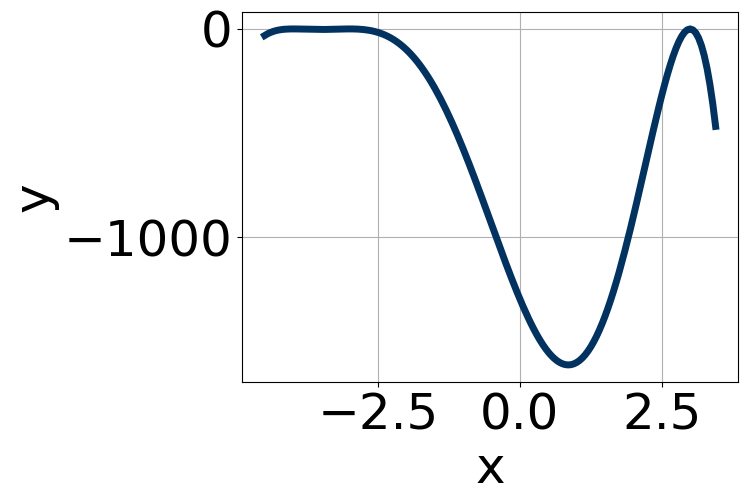
\includegraphics[width=0.5\textwidth]{../Figures/polyGraphToFunctionB.png}
\end{center}
} \newpage
\item{
Construct the lowest-degree polynomial given the zeros below.\[ \frac{-4}{3}, \frac{-5}{3}, \text{ and } -7 \]} \newpage
\item{
Describe the zero behavior of the zero $x = -8$ of the polynomial below.\[ f(x) = -6(x + 2)^{11}(x - 2)^{7}(x + 8)^{3}(x - 8)^{2} \]} \newpage
\item{
Construct the lowest-degree polynomial given the zeros below.\[ \frac{1}{2}, \frac{3}{4}, \text{ and } 4 \]} \newpage
\item{
Describe the end behavior of the polynomial below.\[ f(x) = 2(x + 7)^{4}(x - 7)^{9}(x - 4)^{2}(x + 4)^{2} \]} \newpage
\item{
Construct the lowest-degree polynomial given the zeros below.\[ -2 + 2 i \text{ and } -2 \]} \newpage
\item{
Write an equation that \textit{could} represent the graph below.
\begin{center}
    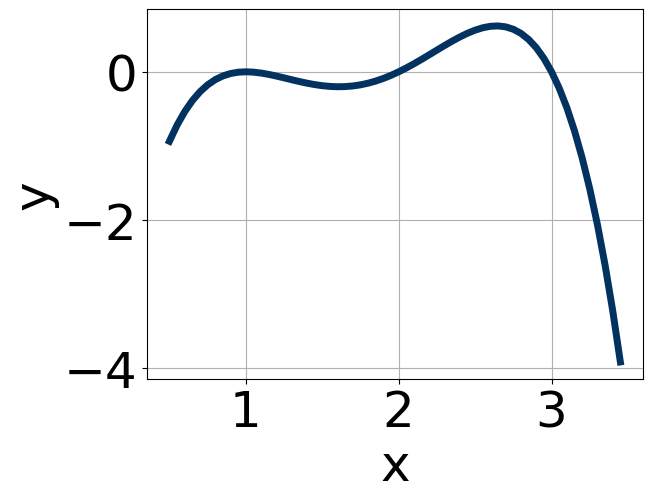
\includegraphics[width=0.5\textwidth]{../Figures/polyGraphToFunctionCopyB.png}
\end{center}
} \newpage
\item{
Construct the lowest-degree polynomial given the zeros below.\[ -2 + 2 i \text{ and } 3 \]} \newpage
\item{
Describe the end behavior of the polynomial below.\[ f(x) = 5(x + 9)^{4}(x - 9)^{7}(x - 7)^{4}(x + 7)^{4} \]} \newpage
\end{enumerate}

\end{document}